\documentclass{../praktikum-protokollvorlage-latex/include/protokollclassE}
\SelectLanguage{english}

\newcommand{\praktikum}{P4}
\newcommand{\semester}{WS18/19}

\newcommand{\wochentag}{Mo}
\newcommand{\gruppennr}{10}

\newcommand{\nachnamea}{Elicabuk}
\newcommand{\vornamea}{Umut}
\newcommand{\nachnameb}{Pittermann}
\newcommand{\vornameb}{Martin}

\input{../common/emails.tex}

\newcommand{\maketitlepage}
{
	\begingroup \let\clearpage\relax
	\tableofcontents
	\listoffigures
	\listoftables
	\endgroup
}

\newcommand{\configureappendix}
{
	\chapter*{\appendixname} \addcontentsline{toc}{chapter}{\appendixname}
}

\newcommand{\s}[1]{\ensuremath{_\text{#1}}}

\DeclareSIUnit{\samples}{S}


\newcommand{\versuch}{Hall Effect}
\newcommand{\betreuer}{Jasmin Seeger}
\newcommand{\durchgefuehrt}{19.11.18}

\newcommand{\abstract}{A hall is a relatively large space enclosed by a roof and walls. Different types of halls have different effects on humans, this phenomenon is known as the \textit{hall effect}. In what follows, we introduce a generalized hall formalism of walls and roofs, ultimately leading to a Grand Unified Hall Theory (GUHT), which is able to describe halls in a general sense.}
\begin{document}
	\FrontMatter
	\include{titlepage.ag}
	\maketitlepage

	\MainMatter

	\chapter{Theory}

\section{Gamma Radiation}
Unlike charged particles, which give off their energy through many interactions by either ionizing other atoms or elastic scattering, gamma rays tend to give off their energy in single bursts by the photoelectric effect (low energies), pair production (high energies) or \textit{Compton scattering} (intermediate energies).

In first order, this leads to a linear relationship between particle energy and distance travelled for charged particles. Thus, they can be shielded entirely.

On the other hand, gamma rays are either absorbed directly by the photoelectric effect or pair production or they change their direction by Compton scattering. Considering a detector pointing in the direction of incident flow, this implies that less gamma rays are detected if an absorber is present, however, gamma rays that do not interact with the absorber still retain their whole initial energy. Therefore, gamma radiation in matter loses intensity but not energy.

For the number of absorbed quanta $\d N$ per path length $\d x$ it holds
\begin{equation}\label{eq:dN}
	\d N = -\mu\cdot N(x)\d x,
\end{equation}
where $\mu$ denotes the \textit{absorption coefficient}.

Integrating \autoref{eq:dN} from 0 to the thickness $d$ of the absorber yields
\begin{equation}\label{eq:Nd}
	N(d) = N_0\cdot\e^{-\mu d},
\end{equation}
where $N_0\equiv N(x=0)$.

As expected, \autoref{eq:Nd} implies that gamma radiation may never be shielded of in its entirety.

\section{The Compton Effect}
\subsection{Differential Cross-Section}
\begin{figure}
	\centering
	\begin{subfigure}{0.49\textwidth}
		\centering
		\includegraphics[width=\textwidth]{example-image-a}
		\caption{s-channel}
		\label{fig:schannel}
	\end{subfigure}
	\begin{subfigure}{0.49\textwidth}
		\centering
		\includegraphics[width=\textwidth]{example-image-b}
		\caption{t-channel}
		\label{fig:tchannel}
	\end{subfigure}
	\par\bigskip
	\begin{subfigure}{0.45\textwidth}
		\centering
		\includegraphics[width=\textwidth]{example-image-c}
		\caption{Kinematic sketch}
		\label{fig:kinematics}
	\end{subfigure}
	\caption{The two tree-level Feynman graphs contributing to the matrix element and a kinematic sketch for Compton scattering}
\end{figure}

The Compton effect is a scattering process of gamma quanta at a free, charged particle. At tree-level, two Feynman graphs (seen in Subfigures \ref{fig:schannel} and \ref{fig:tchannel}) contribute to the Feynman amplitude $\mathcal{M}$.
Denoting the respective 4-momenta of the incident photon and resting electron as
\begin{align*}
	k^\mu &= (k_0\ ,\ \mvec{k}) \\
	p^\mu &= (p_0\ ,\ \mvec{p}),
\end{align*}
and their 4-momenta after the process as primed, using the Feynman rules of QED, we get the two Feynman amplitudes

\begin{align*}
	\mathcal{M}_1 &= \bar{u}^{s'}\left(p'\right)\left(-\iu e\gamma^\nu\right)\epsilon^{*}_\nu\left(k'\right)\left(\frac{\slashed{p}+\slashed{k}+m}{(p+k)^2-m^2}\right)\left(-\iu e\gamma^\mu\right)\epsilon_\mu\left(k\right)u^s(p)\\
	\mathcal{M}_2 &= \bar{u}^{s'}\left(p'\right)\left(-\iu e\gamma^\nu\right)\epsilon_\nu\left(k\right)\left(\frac{\slashed{p}-\slashed{k}+m}{(p-k')^2-m^2}\right)\left(-\iu e\gamma^\mu\right)\epsilon^{*}_\mu\left(k'\right)u^s(p),
\end{align*}
where $u^s(p)$ denotes the incoming electron with spin $s$ and momentum $p^\mu$, $\epsilon^\mu$ is the incident photon's polarization vector and $\gamma^\mu$ are the Dirac matrices.

Since in the canonical formulation of QED the Feynman amplitudes represent terms in the Wick expansion of the perturbative scattering matrix, the total transition amplitude is equal to the sum of these matrix elements
\begin{equation*}
	|\mathcal{M}|^2 = |\mathcal{M}_1|^2 + |\mathcal{M}_2|^2 + 2\Re\left(\mathcal{M}_1\mathcal{M}_2^*\right).
\end{equation*}

For the sake of simplicity (and brevity!), we refer the reader to their QFT textbook of choice and just give the final result in the lab frame
\begin{equation}\label{eq:kleinnishina}
	\frac{\d\sigma}{\d\cos\theta} = \frac{\pi\upalpha^2}{m^2}\left(\frac{\omega'}{\omega}\right)^2\left[\frac{\omega'}{\omega} + \frac{\omega}{\omega'} - \sin^2\theta\right],
\end{equation}
where $m\omega' = \frac{1}{2}\left(m^2-u\right)$ and $m\omega = \frac{1}{2}\left(s-m^2\right)$ and $s=\left(p^\mu + k^\mu\right)^2, s=\left(p^\mu + k'^\mu\right)^2$ are the standard Mandelstam variables.
\autoref{eq:kleinnishina} is known as the \textit{Klein-Nishina formula}.

For electrons bound in an atom, the total cross-section is (in first order) proportional to its atomic number $Z$
\begin{equation*}
	\sigma = Z\cdot\sigma_\text{e}.
\end{equation*}
\subsection{Kinematics}
Consider initial
\begin{align*}
	p^\mu &= (m\ ,\ \mvec{0}) \text{and}\\
	k^\mu &= (E_\gamma\ ,\ \mvec{k})
\end{align*}
and scattered 4-momenta
\begin{align*}
	p'^\mu &= (m\ ,\ \mvec{p}) \text{and}\\
	k'^\mu &= (E'_\gamma\ ,\ \mvec{k'}).
\end{align*}
Using energy
\begin{equation*}
	m + E_\gamma = E'_\text{e} + E'_\gamma,
\end{equation*}
and momentum conservation
\begin{equation*}
	p^2 = E_\text{e}^{'2} - m^2 = \underbrace{E_\gamma^2 + E_\gamma^{'2} - 2E_\gamma E'_\gamma\cos\theta}_\text{law of cosines},
\end{equation*}
yields the energy of the scattered gamma ray
\begin{equation*}
	E'_\gamma = \frac{E_\gamma}{1 + \frac{E_\gamma}{m}\left(1 - \cos\theta\right)}
\end{equation*}
where $E'_\text{e}$ denotes the electron's total energy after the scatter process.

	\chapter{Procedure}
\section{Setup}
The experiment uses a transparent cryostat, a double-walled piece of glassware that is evacuated during the experiment, shown in \autoref{fig:cryostat}.
The probe chamber is located at the end of an elongated section of the cryostat and sits between the poles of a magnetic yoke.
The cryostat is cooled with liquid nitrogen, which is held in a toroidal storage tank.
The probe chamber is connected to the storage tank via a small tube, the flow of liquid nitrogen is limited by the static pressure due to nitrogen evaporating in the probe chamber.
Venting the probe chamber with the topmost valve regulates the pressure and in turn the flow of liquid nitrogen.

To examine the Hall effect, a superconducting coil is used to set the magnetic field of the samples.

A heating coil, which is regulated by a PID controller, is used to accurately set the temperature of the probe chamber.
This gives a total temperature range of \SIrange{-180}{150}{\celsius} for the experiment.

For each temperature, four measurements are recorded: the current through the sample $I$, the longitudinal voltage $U_\text{L}$ with no external magnetic field and the hall voltage $U_\text{H}^{+,-}$ at a magnetic field of $B = \pm \SI{0.5}{\tesla}$.

\begin{figure}
	\centering
	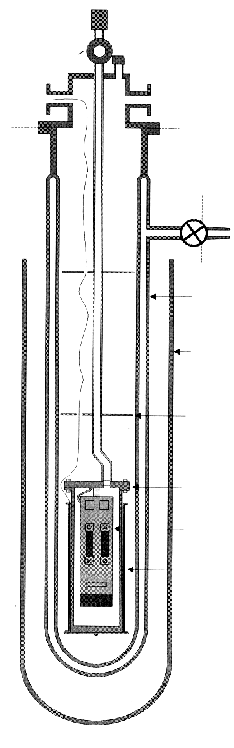
\includegraphics[width=.7\textwidth]{./img/cryostat.png}i
	\caption[Cryostat]{The cryostat used in the experiment}
	\label{fig:cryostat}
\end{figure}

\section{Samples}
\subsection{Sample A (Ge)}
Sample A is a platelet of germanium of dimensions \SI{19}{\mm} x \SI{10}{\mm} x \SI{1}{\mm}.
Contacts are made with thin gold wires, which are attached to electrolytically gold plated areas of the sample.
The exact geometry is shown in \autoref{fig:samples:ge}.

\subsection{Sample B (GaAs 2DEG)}
Sample B is considered to be a 2D electron gas inside a GaAs heterostructure.
The individual layers are depicted in the cross section \autoref{fig:samples:gaas-cross}.
The 2DEG forms between the active GaAs layer and the n-doped layer of AlGaAs.
The macroscopic shape of the sample is shown in \autoref{fig:samples:gaas-clover}.

The clover leaf or cross shaped geometry is chosen to minimize errors introduced by effects of the imperfect metal-semiconductor contact, as discussed in \autoref{sec:van-der-pauw-geometry}. Thanks to the design provided in this experiment, probing points that are necessary to measure value pairs $\left(V_\text{long}, I_\text{diag}\right)$ and $\left(V_\text{H}, I_\text{long}\right)$ can be selected by the flick of a switch.

The electron density $n_\text{2D}$ and mobility $\mu$, as stated by the manufacturer, are listed in \autoref{tab:lit-2deg}.

\begin{table}
	\centering
	\caption{Parameters of the 2DEG (stated by the manufacturer)}
	\label{tab:lit-2deg}
	\begin{tabular}{SSS}
		\toprule
		{$T$ (\si{\kelvin})}&	{$n_\text{2D}$ (\si{\per\centi\meter\squared})}&	{$\mu$ (\si{\centi\meter\squared\per\volt\per\second})}\\
		\midrule
		300&	2.9e11&	6.5e2\\
		70&	1.7e11&	1.94e5\\
		\bottomrule
	\end{tabular}
\end{table}

\begin{figure}
	\centering
	\begin{subfigure}{0.45\textwidth}
		\centering
		\includegraphics[width=\textwidth]{./img/sample-ge.png}
		\caption{Sample A (Ge)}
		\label{fig:samples:ge}
	\end{subfigure}
	\begin{subfigure}{0.45\textwidth}
		\centering
		\includegraphics[width=\textwidth]{./img/sample-gaas-clover.png}
		\caption{Sample B (GaAs)}
		\label{fig:samples:gaas-clover}
	\end{subfigure}
  \par\bigskip
	\begin{subfigure}{0.7\textwidth}
		\centering
		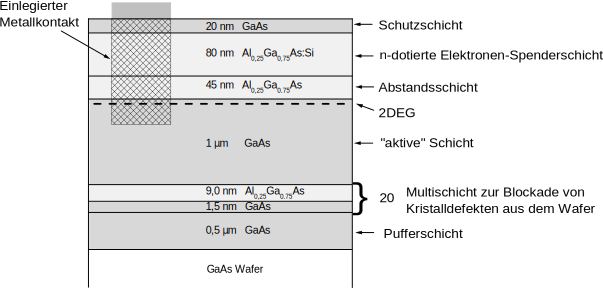
\includegraphics[width=\textwidth]{./img/sample-gaas-cross.pdf}
		\caption{Sample B (GaAs) cross section}
		\label{fig:samples:gaas-cross}
	\end{subfigure}
	\caption{The samples used in the experiment}
\end{figure}

	\chapter{Analysis of Data}

\section{Sample A}

\section{Sample B}

\section{Comparison of Hall Mobilities}
\begin{figure}
  \centering
  \includegraphics[width=.6\textwidth]{./data/plots/mob-comp.pdf}
  \captiond{Comparison of hall mobility for both samples}{}
  \label{fig:mob-comp}
\end{figure}

Hall mobility dependences for both samples are compared in \autoref{fig:mob-comp}.
Apart from their obviously different absolute values, it is easy to see that the curves exhibit different temperature dependencies for low temperatures (with respect to the observed temperature range).

\textbf{The germanium sample (A)} shows a temperature dependence which is in accordance with the theory outlined in \autoref{subsec:phonons}: For high temperatures, scattering at acoustic phonons makes a major contribution to the hall mobility $\left(T^{-\nicefrac{3}{2}}\right)$.
For low temperatures, scattering at charged defects results in a $\propto T^{\nicefrac{3}{2}}$ behavior.

\textbf{The GaAs composite sample (B)} appears to show the expected behavior as well.
For this temperature regime, scattering at optical phonons should make the main contribution to the overall behavior so that a behavior like $\mu\propto \e^\frac{\hbar \omega}{k T} - 1$ is expected.
This assumption is confirmed by the observed data.

	%\Appendix
\configureappendix

\section{Calculation of Differential Cross-Section}\label{appendix:cross}

To obtain the differential cross-section depicted in \autoref{fig:diff_cross}, first, the remaining gamma ray flux at the target has to be calculated since the activity of the source decays over time.
The lab manual specifies a gamma ray flux of $\phi_0 = \SI{1.54(9)e6}{\per\cm\squared\per\second}$ for the $^{137}$Cs source.
The reference measurement from the lab manual was conducted in July, 1971.
Since no day was specified, the middle of July is assumed.

Under these assumptions, the remaining gamma ray flux is
\begin{equation*}
	\phi_\text{rem} = \phi_0\cdot\exp\left(\frac{t_\text{init}-t_\text{exp}}{t_{\nicefrac{1}{2}}}\right),
\end{equation*}
where $t_\text{init}-t_\text{exp}$ denotes the timespan (in days) between the reference and the experiment conducted in this lab report.
$t_{\nicefrac{1}{2}}$ is the half-life of the $^{137}$Cs source in days.
The specified error is propagated like
\begin{equation*}
	\sigma_{\phi\text{, rem}} = \sigma_{\phi,0}\cdot\exp\left(\frac{t_\text{init}-t_\text{exp}}{t_{\nicefrac{1}{2}}}\right).
\end{equation*}

The volume of the Al target is
\begin{equation*}
	V = \ell\cdot\pi\cdot\left(\frac{d}{2}\right)^2,
\end{equation*}
where $\ell=\SI{1.0(1)}{\cm}$ and $d=\SI{1.0(1)}{\cm}$ denote the length and diameter of the target, respectively.

	%\TheBibliography
\bibliographystyle{alpha}
\bibliography{../common/lit}

\end{document}
